\section{Determinação do seno, cosseno e tangente}
	\begin{figure}[H]
		\caption{Determinação do seno, cosseno e tangente}
		\label{triangulo_retangulo}
		\centering
		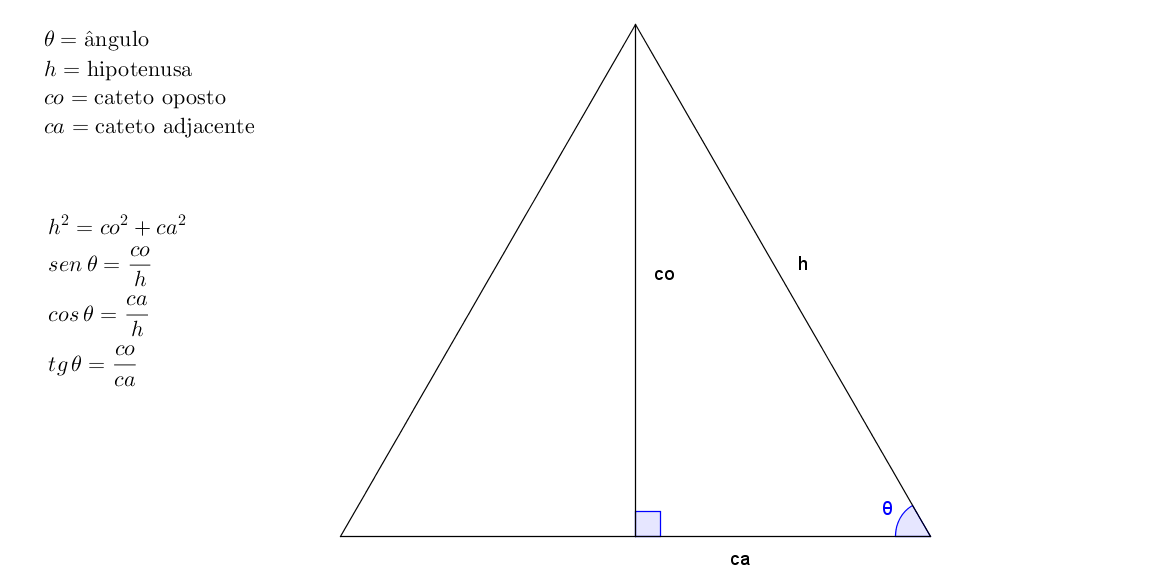
\includegraphics[width=\textwidth]{triangulo_retangulo.png}		
	\end{figure}
	
\section{Círculo trigonométrico}
	\begin{figure}[H]
		\caption{Círculo trigonométrico}
		\label{circulo_trigonometrico}
		\centering
		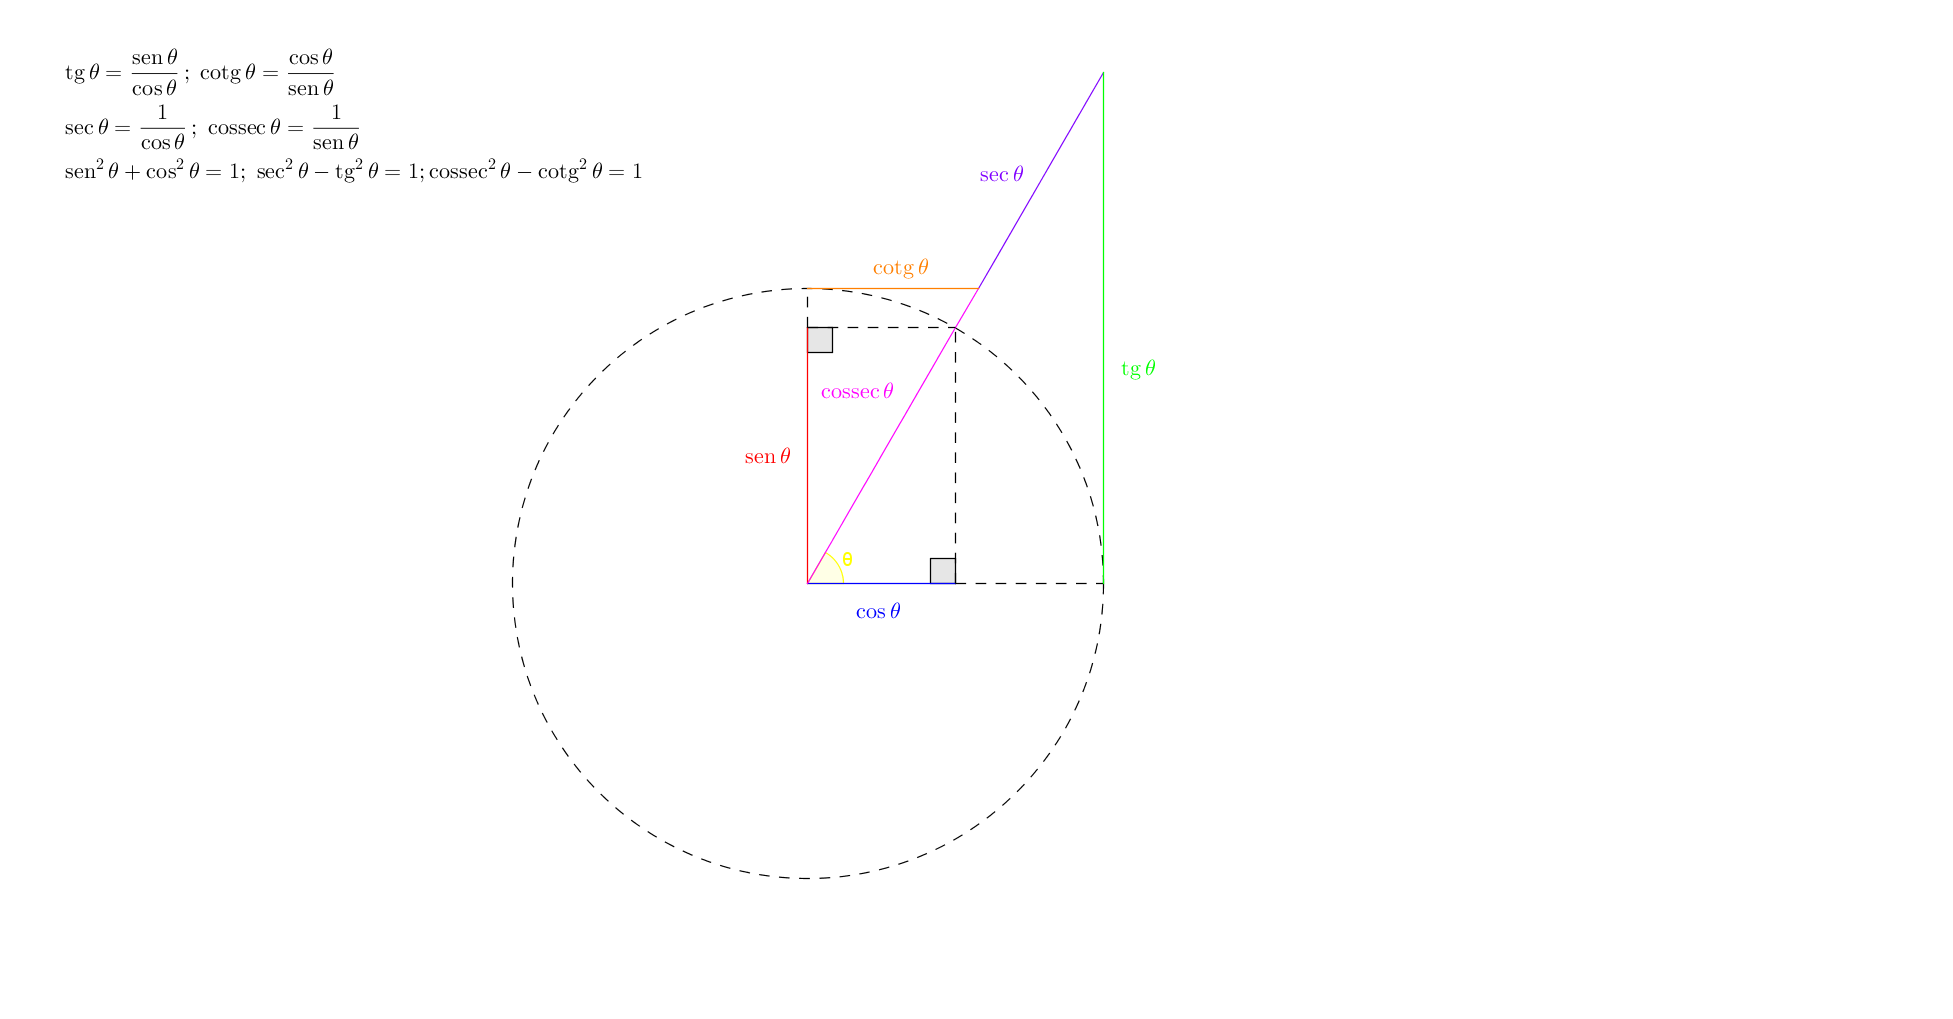
\includegraphics[width=\textwidth]{circulo_trigonometrico.png}		
	\end{figure}
	
\section{Identidades trigonométricas}
	\begin{table}[H]
		\caption{Identidades trigonométricas}
		\label{identidades_trigonometricas}
		\centering
		\begin{tabular}{|lcl|}
			$\tg(x)$                    & $=$ & $\dfrac{\sen(x)}{\cos(x)}$ \\
			$\cotg(x)$                  & $=$ & $\dfrac{\cos(x)}{\sen(x)}$ \\
			$\sec(x)$                   & $=$ & $\dfrac{1}{\cos(x)}$       \\
			$\cossec(x)$                & $=$ & $\dfrac{1}{\sen(x)}$       \\
			$\sen^2(x) + \cos^2(x)$     & $=$ & $1$                        \\
			$\sec^2(x) - \tg^2(x)$      & $=$ & $1$                        \\
			$\cossec^2(x) - \cotg^2(x)$ & $=$ & $1$                        \\
			$\sen^2(x)$                 & $=$ & $\dfrac{1 - \cos(2x)}{2}$  \\
			$\cos^2(x)$                 & $=$ & $\dfrac{1 + \cos(2x)}{2}$  \\
			$\sen(2x)$                  & $=$ & $2\sen(x)\cos(x)$          \\
			$\cos(2x)$                  & $=$ & $\cos^2(x) - \sen^2(x)$
		\end{tabular}		
	\end{table}
	
\section{Relação entre trigonométricas e inversas}
	\begin{table}[H]
		\caption{Relação entre trigonométricas e inversas}
		\label{relacao_trigonometricas_inversas}
		\centering
		\begin{tabular}{|lclclcl|}
			$\sen (\theta)$    & $=$ & $x$ & $\Rightarrow$ & $\theta$ & $=$ & $\arcsen (x)$    \\
			$\cos (\theta)$    & $=$ & $x$ & $\Rightarrow$ & $\theta$ & $=$ & $\arccos (x)$    \\
			$\tg (\theta)$     & $=$ & $x$ & $\Rightarrow$ & $\theta$ & $=$ & $\arctg (x)$     \\
			$\cossec (\theta)$ & $=$ & $x$ & $\Rightarrow$ & $\theta$ & $=$ & $\arccossec (x)$ \\
			$\sec (\theta)$    & $=$ & $x$ & $\Rightarrow$ & $\theta$ & $=$ & $\arcsec (x)$    \\
			$\cotg (\theta)$   & $=$ & $x$ & $\Rightarrow$ & $\theta$ & $=$ & $\arccotg (x)$
		\end{tabular}		
	\end{table}

\section{Substituição trigonométrica}
	\begin{table}[H]
		\caption{Substituição trigonométrica}
		\label{substituicao_trigonometrica}
		\centering
		\begin{tabular}{|lclcl|}
			$\sqrt{a^2 - x^2}$ & $\Rightarrow$ & $x$ & $=$ & $a\sen (\theta)$ \\
			$\sqrt{a^2 + x^2}$ & $\Rightarrow$ & $x$ & $=$ & $a\tg (\theta)$  \\
			$\sqrt{x^2 - a^2}$ & $\Rightarrow$ & $x$ & $=$ & $a\sec (\theta)$
		\end{tabular}		
	\end{table}

\section{Ângulos notáveis}
	\begin{table}[H]
		\caption{Ângulos notáveis}
		\label{angulos_notaveis}
		\centering
		\begin{tabular}{|l|l|l|l|l|l|}
			\hline
			ângulo & $0^\circ\, (0)$ & $30^\circ\, \left(\frac{\pi}{6}\right)$ & $45^\circ\, \left(\frac{\pi}{4}\right)$ & $60^\circ\, \left(\frac{\pi}{3}\right)$ & $90^\circ\, \left(\frac{\pi}{2}\right)$ \\ \hline
			$\sen$ & $0$             & $\dfrac{1}{2}$                          & $\dfrac{\sqrt{2}}{2}$                   & $\dfrac{\sqrt{3}}{2}$                   & $1$                                     \\ \hline
			$\cos$ & $1$             & $\dfrac{\sqrt{3}}{2}$                   & $\dfrac{\sqrt{2}}{2}$                   & $\dfrac{1}{2}$                          & $0$                                     \\ \hline
			$\tg$  & $0$             & $\dfrac{\sqrt{3}}{3}$                   & $1$                                     & $\sqrt{3}$                              & $\nexists$                                \\ \hline
		\end{tabular}		
	\end{table}